% 03.1. ASPECTOS ARQUITECTURALES Y TECNOLOGICOS
%----------------------------------------------------------------------------------------------
El patrón que vamos a utilizar para el diseño arquitectural de nuestro 
catálogo va a ser el de Modelo-Vista-Controlador, en concreto, la variante Modelo-Vista-Presentador (véase la~\cref{fig:diagDespliegue}).

\vspace{.2cm}
\begin{figure}[ht]
	\centerline{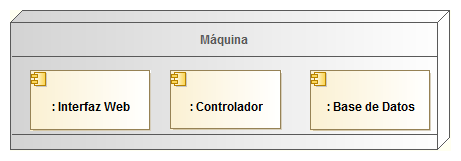
\includegraphics[scale=0.6]{img/diagrama_despliegue}}\
	\caption{Diagrama de despliegue del sistema}
	\label{fig:diagDespliegue}
\end{figure}


\paragraph{Interfaz web.} Es nuestro componente vista, lo que utilizan los usuarios para 
interactuar con la aplicación y visualizar los resultados que producen dichas
interacciones. Las acciones del usuario que impliquen el acceso o la modificación
de los datos del modelo son delegadas al componente Controlador.

\paragraph{Controlador.} Es nuestro componente Presentador, tiene toda la lógica de la vista 
y es responsable de sincronizar el modelo y la vista. Cuando la vista notifica el 
presentador que el usuario ha hecho algo (por ejemplo, hacer clic en un botón), 
el presentador a continuación, actualiza el modelo y sincroniza los cambios 
entre el modelo y la vista.

\paragraph{Base de datos.} Es nuestro componente modelo, se encarga de encapsular 
los datos y ofrecer operaciones para su acceso y procesamiento. Solo el componente
Controlador interactúa con este componente.\newline\newline
Las tecnologías utilizadas son las que se detallaron en el apartado anterior.